\documentclass[aspectratio=169]{beamer}


\usetheme{metropolis} 
\usepackage[style=verbose-note, url=true]{biblatex}
\usepackage{graphicx,microtype,geometry,listings}
\addbibresource{main.bib}

% Presentation information
\title{OTel Without Reservations}
\author{Ethan Kent}
\date{\today}

\begin{document}

\begin{frame}
  \titlepage
\end{frame}

\begin{frame}{Overview}
  \tableofcontents
\end{frame}

\section{Let's dive right in}

\begin{frame}{What is OpenTelemetry?}
  \begin{enumerate}
    \item Follow the steps at https://opentelemetry.io/docs/instrumentation/js/getting-started/nodejs/.
    \item Follow the steps at https://opentelemetry.io/docs/instrumentation/js/exporters/.
    \item Follow the steps at https://opentelemetry.io/docs/instrumentation/js/manual/\#acquiring-a-tracer.
    \item Show prepared demo that adds DB calls.
  \end{enumerate}


  \lstinline[basicstyle=\tiny]{docker run --name some-postgres -p 5432:5432 -e POSTGRES_PASSWORD=mysecretpassword -d postgres}
\end{frame}

\section{Introduction}
\begin{frame}{What is OpenTelemetry?}

  According to the OpenTelemetry people,\footnote{OpenTelemetry is a project of
    The Cloud Native Computing Foundation and is a merger of the OpenTracing and
    OpenCensus projects.}

  \vspace{1em}

  \begin{quote}
    OpenTelemetry is a collection of tools, APIs, and SDKs. Use it to
    instrument, generate, collect, and export telemetry data (metrics, logs, and
    traces) to help you analyze your software's performance and
    behavior.\footcite{otel-site}
  \end{quote}
\end{frame}

\begin{frame}{Why do I care?}
  \begin{quote}

    A \emph{distributed trace}, more commonly known as a \emph{trace}, records
    the paths taken by requests (made by an application or end-user) as they
    propagate through multi-service architectures, like microservice and
    serverless applications.

    \vspace{0.618em}

    Without tracing, it is challenging to pinpoint the cause of performance
    problems in a distributed system.

    \vspace{0.618em}

    It improves the visibility of our application or system's health and lets us
    debug behavior that is difficult to reproduce locally. Tracing is essential
    for distributed systems, which commonly have nondeterministic problems or are
    too complicated to reproduce locally.\footcite{otel-dist-trace}

  \end{quote}
\end{frame}

\begin{frame}{Why do I care? (cont'd)}
  \begin{center}
    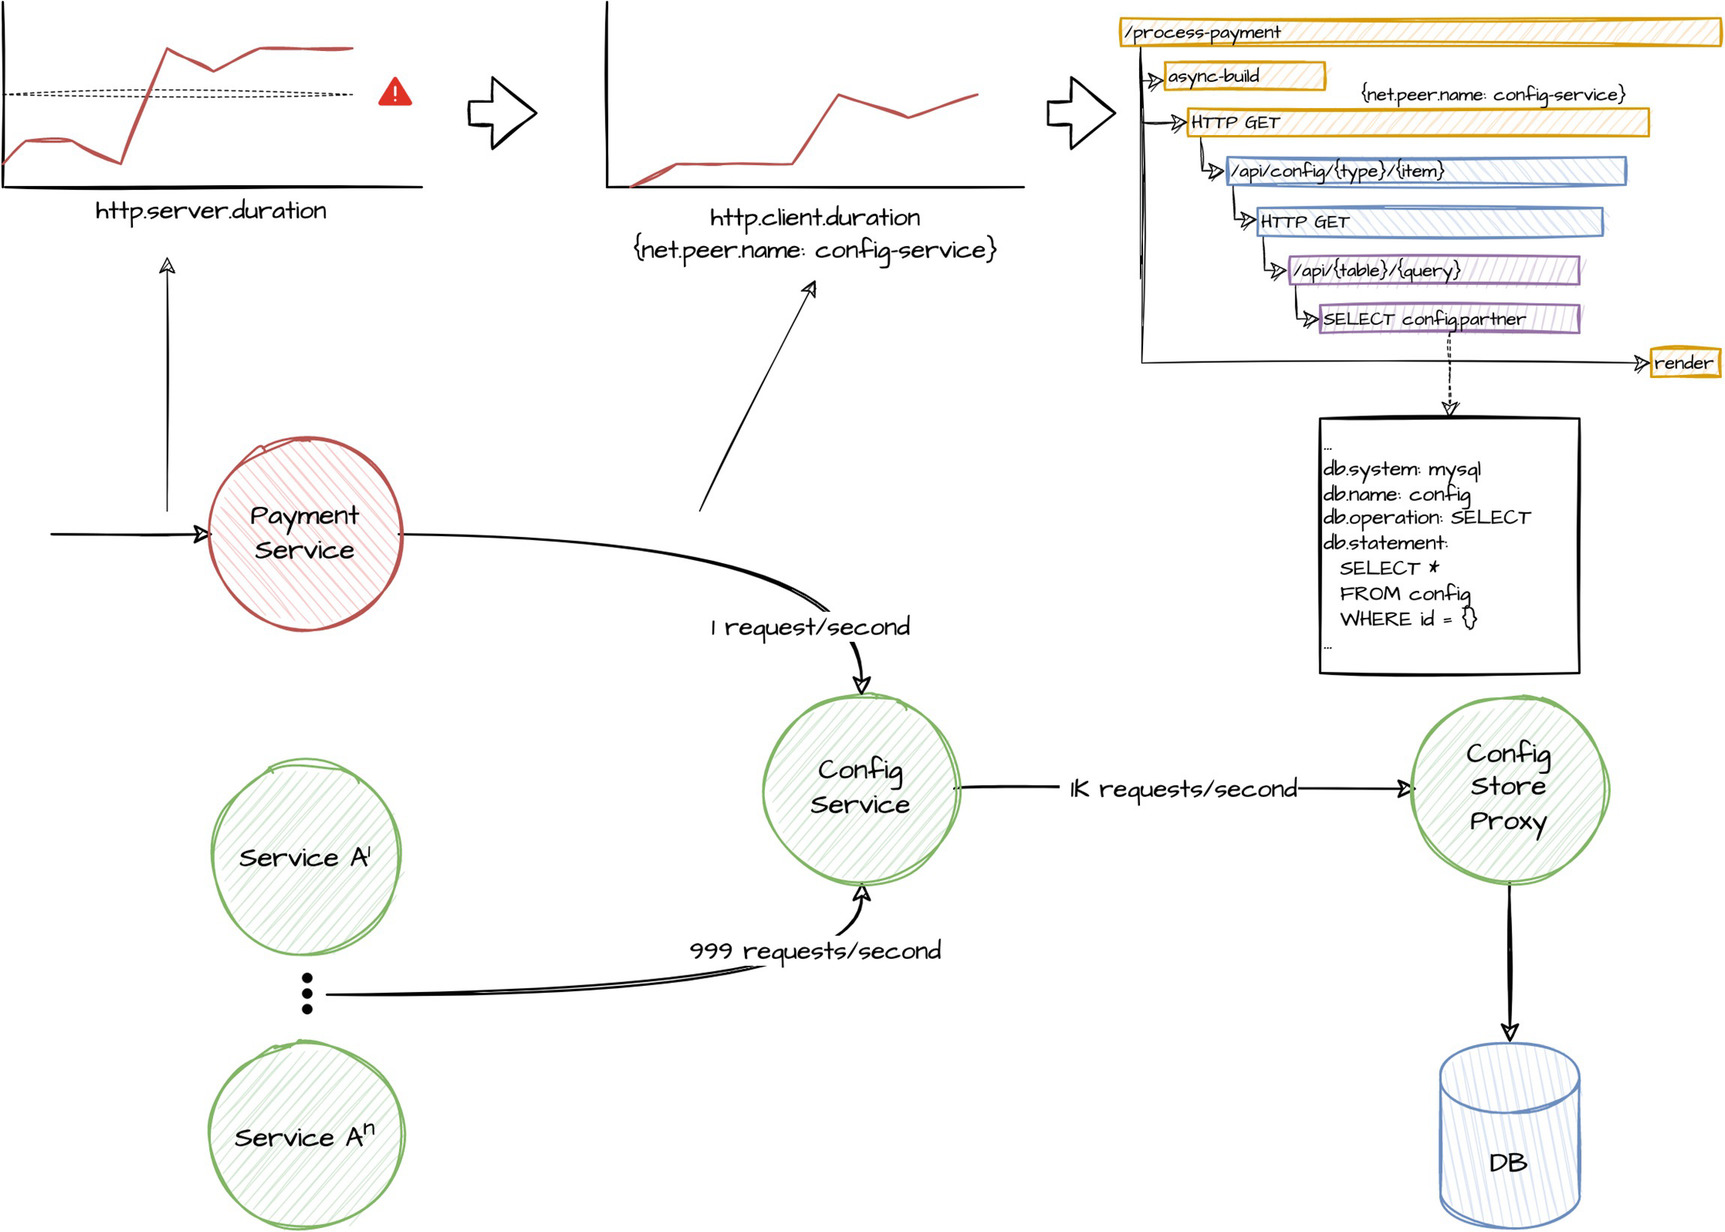
\includegraphics[width=0.9\textwidth, height=0.9\textheight, keepaspectratio]{distributed-tracing.jpg}
  \end{center}
\end{frame}

\begin{frame}{Why do I care? (cont'd)}
  \begin{description}
    \item[Observability] OpenTelemetry (OTel) offers comprehensive observability
      across your systems. OTel provides a clear picture of what's happening
      within your services by bringing together traces, metrics, and logs.
    \item[Reduced Complexity] OTel unifies multiple observability signals into a
      coherent framework. A single framework simplifies instrumentation and
      eliminates the need to learn and manage various systems.
    \item[Standards-Based] OTel is open-source and vendor-neutral, providing
      standardized APIs and instrumentation that integrates with any backend.
    \item[Extensibility] OTel's modular design allows you to use what you need,
      and its SDKs let you build custom integrations as required.
    \item[Cost and Resource Efficient] OTel can reduce the overhead and costs of
      running multiple observability tools.
  \end{description}
\end{frame}

\begin{frame}{Why do I care? (cont'd)}
  \begin{description}
    \item[Support for Modern Architectures] OTel provides first-class support
      for Kubernetes, serverless functions, and service meshes.
    \item[Enhanced Debugging] With better visibility, engineers can identify,
      understand, and resolve issues faster.
    \item[Performance Monitoring] OTel helps you monitor system performance and
      user behavior in real time, helping you make data-driven decisions to
      improve your services' performance and user experience.
    \item[Future-Proof] OTel's wide adoption and large community likely mean
      that as new standards and best practices emerge, OTel will evolve with them.
  \end{description}
\end{frame}

\section{Signals}

\begin{frame}{Signals}
  ``In OpenTelemetry, a signal refers to a category of telemetry.''\footcite{otel-signals}

  \vspace{1em}

  The four kinds of signals currently supported are

  \begin{itemize}
    \item Traces,
    \item Metrics,
    \item Logs, and
    \item Baggage.\footcite{otel-signals}
  \end{itemize}
\end{frame}

\begin{frame}{Traces}
  \emph{Spans} are the bread and butter of distributed tracing. A \emph{Trace}
  has many \emph{Spans}.

  \vspace{1em}

  \begin{quote}
    Traces give us the big picture of what happens when a request is made to an
    application. Whether your application is a monolith with a single database
    or a sophisticated mesh of services, traces are essential to understanding
    the full ``path'' a request takes in your application.\footcite{otel-traces}
  \end{quote}
\end{frame}

\begin{frame}{Metrics}

  \begin{quote}

    A metric is a measurement about a service, captured at runtime. Logically,
    the moment of capturing one of these measurements is known as a metric event
    which consists not only of the measurement itself, but the time that it was
    captured and associated metadata.\footcite{otel-metrics}

  \end{quote}
\end{frame}

\begin{frame}{Metrics (cont'd)}

  Use metrics when you want metrics.

  \vspace{1em}

  \begin{quote}

    Some telemetry backends allow to execute ad hoc queries on spans, [and it]
    is also possible to derive metrics from spans in OpenTelemetry Collectors.
      {\Large This often results in an overuse of spans as a substitute for
        metrics when teams start to adopt tracing.} Trace sampling can affect any
    interpretations extracted directly from spans,~.~.~. [and] the high volumes
    of data and cardinality processed by trace pipelines in high-throughput
    systems normally result in signals that are less stable than metrics
    originating directly from a service~.~.~.~.\footcite[ch.~6, emphasis
      added]{practical-otel}

  \end{quote}
\end{frame}

\begin{frame}{Logs}
  \begin{quote}

    In OpenTelemetry, any data that is not part of a distributed trace or a
    metric is a log. For example, events are a specific type of log. Logs often
    contain detailed debugging/diagnostic info, such as inputs to an operation,
    the result of the operation, and any supporting metadata for that
    operation.\footcite{otel-logs}

  \end{quote}
\end{frame}

\begin{frame}{Logs: not well-supported yet}
  \begin{center}
    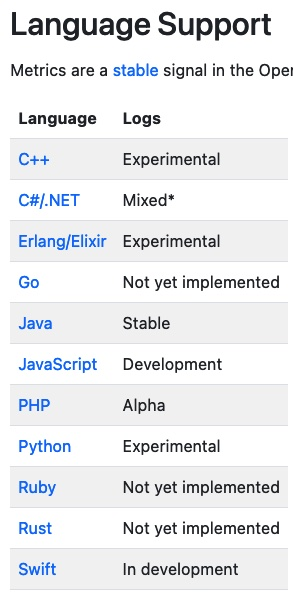
\includegraphics[height=0.8\textheight]{logs-support.jpg}
  \end{center}
\end{frame}

\begin{frame}{Baggage}
  ``In OpenTelemetry, Baggage is contextual information that's passed between
  spans. It's a key-value store that resides alongside span context in a trace,
  making values available to any span created within that trace.''\footcite{otel-baggage}

  It's in the HTTP headers, so don't store sensitive data.

  ``Common use cases include~.~.~. Account Identification, User Ids, Product
  Ids, and origin IPs.~.~.~. Passing these down your stack allows you to then
  add them to your Spans in downstream services to make it easier to filter when
  you're searching in your Observability back-end.''\footcite{otel-baggage}
\end{frame}

\section{Context and Context Propagation}

\begin{frame}{How does this distributed stuff work?}

  Distributed tracing is hard because it's tricky to reconstruct
  cause-and-effect relationships. In distributed systems, many separate
  services---some internal and some external---may collaborate to produce a
  final result. The secret sauce for OpenTelemetry can be split into three
  pieces:

  \begin{enumerate}
    \item A trace ID, additional correlation IDs, and other metadata,
          collectively called ``Context.''
    \item Standards governing how Context is transmitted within and among
          services, called ``Context Propagation.''
    \item An ecosystem comprising open standards, libraries, SDKs, vendors, etc.
  \end{enumerate}

  \vspace{1em}

  In short, OpenTelemetry is a well-thought-out system for assigning IDs in a
  tree-like structure, passing them across service boundaries, and then allowing
  Humpty-Dumpty to be put back together again.

\end{frame}

\begin{frame}{Context}
  \begin{quote}

    In order for OpenTelemetry to work, it must store and propagate important
    telemetry data. For example, when a request is received and a span is
    started it must be available to a component which creates its child span. To
    solve this problem, OpenTelemetry stores the span in the
    Context.\footcite{otel-context-js}

  \end{quote}
\end{frame}

\begin{frame}{Context (cont'd)}
  \begin{quote}

    A \lstinline{Context} is a propagation mechanism which [sic] carries
    execution-scoped values across API boundaries and between logically
    associated execution units. Cross-cutting concerns access their data
    in-process using the same shared \lstinline{Context}
    object.\footcite{otel-context}

  \end{quote}

  \vspace{1em}

  \begin{quote}

    \begin{description}
      \item[Execution Unit] An umbrella term for the smallest unit of sequential
        code execution, used in different concepts of multitasking. Examples are
        threads, coroutines or fibers.\footcite{otel-defs}
    \end{description}

  \end{quote}

\end{frame}

\begin{frame}{Context Propagation}
  Context Propagation

  \vspace{1em}

  \begin{quote}

    Propagation is the mechanism that moves data between [sic] services and
    processes. Although not limited to tracing, it is what allows traces to
    build causal information about a system across services that are arbitrarily
    distributed across process and network
    boundaries.\footcite{otel-propagation}

  \end{quote}
\end{frame}


\begin{frame}{Context Propagation (cont'd)}

  You can think of a \lstinline{Propagators} as serializers/deserializers or
  marshallers/unmarshallers for \lstinline{Context}.

  \begin{quote}

    Cross-cutting concerns send their state to the next process using
    \lstinline{Propagators}, which are defined as objects used to read and write
    context data to and from messages exchanged by the applications. Each
    concern creates a set of \lstinline{Propagators} for every supported
    Propagator type.\footcite{otel-propagators}

  \end{quote}
\end{frame}

\section{API, SDK, and Semantic Conventions}

\begin{frame}{API and SDK}

  Remember my talks on Onion Architecture and SOLID, specifically the
  Dependency-Inversion Principle? What, you think you can pick up in Season 3
  and not miss anything?

  \vspace{1em}

  Okay, VERY BRIEFLY THEN.

\end{frame}

\section{Brief aside, wherein Ethan gets back up on his Dependency-Inversion soapbox}

\begin{frame}[fragile]{Not dependency inverted}
  \begin{lstlisting}[basicstyle=\footnotesize]
class MyBusinessLogic {
  private logger: ConsoleLogger;
  private businessDataWriter: MySqlBusinessDataWriter;

  constructor() {
    this.logger = new ConsoleLogger();
    this.businessDataWriter = new MySqlBusinessDataWriter();
  }

  public processBusinessData(businessData: BusinessData) {
    this.businessDataWriter
      .writeBusinessData(businessData)
      .then(() => this.logger.logDebug("It worked fine"))
      .catch((e) => this.logger.logError(`We had a problem: ${e}`));
  }
}
  \end{lstlisting}
\end{frame}

\begin{frame}{Not dependency inverted (cont'd)}

  Requirements change, hotshot: let's use Pino instead of the
  \lstinline{console} to do logging, and let's use \lstinline{PostgreSQL}
  instead of \lstinline{MySql} for storing the data.

  \vspace{1em}

  Should the implementation have to change for our business-logic class if only
  the dependencies, not the business logic, changed?

  \vspace{1em}

  Can you do that without changing the innards of \lstinline{MyBusinessLogic} as
  presently written? Does this violate the Dependency-Inversion Principle? Does
  it violate the Open--Closed Principle? Does a business stakeholder now
  potentially have to care about your database or logging choice?

  \vspace{1em}

  Answer Key: No (uh-oh) \\
  No (whoops), Yes (whoops), Yes (whoops), Yes (whoops).

\end{frame}


\begin{frame}[fragile]{Dependency inverted}
  \begin{lstlisting}[basicstyle=\footnotesize]
type LoggingService = {
  logDebug: (message: string) => void;
  logError: (message: string) => void;
};

type BusinessDataWriterService = {
  writeBusinessData: (businessData: BusinessData) => Promise<void>;
};
  \end{lstlisting}
\end{frame}

\begin{frame}[fragile]{Dependency inverted (cont'd)}
  \begin{lstlisting}[basicstyle=\footnotesize]
class MyBusinessLogic {
  constructor(
    private logger: LoggingService,
    private businessDataWriter: BusinessDataWriterService
  ) {}

  public processBusinessData(businessData: BusinessData) {
    this.businessDataWriter
      .writeBusinessData(businessData)
      .then(() => this.logger.logDebug("It worked fine"))
      .catch((e) => this.logger.logError(`We had a problem: ${e}`));
  }
}
  \end{lstlisting}
\end{frame}


\begin{frame}[fragile]{Dependency inverted (cont'd)}
  \begin{lstlisting}[basicstyle=\footnotesize]
// New file pino-logger.ts
class PinoLogger implements LoggingService { /* ...impl */ }

// New file postgres-sql-writer.ts
class PostgreSqlBusinessDataWriter implements BusinessDataWriterService {
  /* ...impl */ 
}

// In main.ts, update this
new MyBusinessLogic(new ConsoleLogger(), new MySqlBusinessDataWriter());

// to this
new MyBusinessLogic(new PinoLogger(), new PostgreSqlBusinessDataWriter());
  \end{lstlisting}
\end{frame}

\begin{frame}{Dependency inverted (cont'd)}

  Requirements change, hotshot: let's use Pino instead of the
  \lstinline{console} to do logging, and let's use \lstinline{PostgreSQL}
  instead of \lstinline{MySql} for storing the data.

  \vspace{1em}

  Should the implementation have to change for our business-logic class if only
  the dependencies, not the business logic, changed?

  \vspace{1em}

  Can you do that without changing the innards of \lstinline{MyBusinessLogic} as
  presently written? Does this violate the Dependency-Inversion Principle? Does
  it violate the Open--Closed Principle? Does a business stakeholder now
  potentially have to care about your database or logging choice?

  \vspace{1em}

  Answer Key: Heck no! \\
  heck yes, heck no, heck no, heck no.

\end{frame}

\begin{frame}{Dependency inverted (cont'd)}

  How did we do this?

  \vspace{1em}

  \begin{quote}

    Abstractions should not depend on details. Details (concrete
    implementations) should depend on abstractions.\footcite{enwiki:1148320529}

  \end{quote}

\end{frame}

\section{API, SDK, and Semantic Conventions, resumed}

\begin{frame}{API and SDK (cont'd)}
  The API is the dependency-inverted abstraction. Remember, depend on
  abstractions.

  \vspace{1em}

  \begin{quote}

    API packages consist of the cross-cutting public interfaces used for
    instrumentation. Any portion of an OpenTelemetry client which is imported
    into third-party libraries and application code is considered part of the
    API.\footcite{otel-overview}

  \end{quote}

\end{frame}

\begin{frame}{API and SDK (cont'd)}

  The SDK is the dependency-inverted set of concretions. The actual
  implementations.

  \vspace{1em}

  \begin{quote}

    The SDK is the implementation of the API provided by the OpenTelemetry
    project. Within an application, the SDK is installed and managed by the
    application owner. Note that the SDK includes additional public interfaces
    which are not considered part of the API package, as they are not
    cross-cutting concerns. These public interfaces are defined as constructors
    and plugin interfaces. Application owners use the SDK constructors; plugin
    authors use the SDK plugin interfaces. Instrumentation authors MUST NOT
    directly reference any SDK package of any kind, only the
    API.\footcite{otel-overview}

  \end{quote}
\end{frame}

\begin{frame}{Semantic Conventions}

  ``Semantic Conventions'' is the name for what amounts to a set of constants
  specified to allow naming things consistently. They live in their own repo,
  https://github.com/open-telemetry/semantic-conventions.

\end{frame}

\section{Practical Use of OpenTelemetry}
\begin{frame}{Auto Instrumentation}

  \begin{quote}

    \textbf{Zero-touch model}: The instrumented application code is unchanged,
    and the OpenTelemetry SDK and instrumentation libraries are initialized by a
    separate component and configured independently from the instrumented code.
    This model is the easiest one to implement for service owners, but it's not
    available in every language and normally requires being able to modify the
    command used to start the application, for example, attaching the Java agent
    or using Python's \lstinline{telemetry-instrument} command, or having access
    to configure the runtime environment as in .NET's CLR profiler. In some
    cases, this model can limit the options to configure or customize certain
    aspects of instrumentation libraries.\footcite[ch.~4]{practical-otel}

  \end{quote}

\end{frame}

\begin{frame}{Manual Instrumentation}

  \textbf{Implementation model}: The OpenTelemetry SDK and instrumentation
  libraries are configured and initialized by the application owner as part of the
  instrumented application code, normally happening during application startup.
  This may provide more flexibility to configure instrumentations, but it requires
  extra effort to install and maintain. In some languages, like Java, this model
  can have additional drawbacks, as instrumentation libraries that dynamically
  inject bytecode in the agent model cover a wider set of instrumented libraries
  and frameworks.\footcite[ch.~4]{practical-otel}

\end{frame}

\begin{frame}{Automatic v.~Manual Instrumentation}

  In practice, a combination of both may be used, with auto instrumentation
  covering standard libraries and frameworks, and manual instrumentation filling
  in the gaps for custom or unsupported libraries, or for more granular control
  over spans and attributes.

\end{frame}

\section{Justin with some DevOps perspective}

\end{document}